\documentclass{article}
\usepackage{fullpage}
\usepackage{hyperref}
\hypersetup{colorlinks}
\hyphenpenalty=100000
\usepackage{graphicx}
\DeclareGraphicsExtensions{.pdf,.png,.jpg}
\begin{document}
\setlength{\voffset}{3.5in}
\title{Milestone 5}
\author{Super Smash Bros Brawl Management System \\
Team Shine: Seth RanChao Zhang, Trevor Krenz, and Richard Thai}
\date{16 February 2012}
\maketitle
\clearpage
\setlength{\voffset}{0pt}
\tableofcontents
\clearpage
\section{Executive Summary}
This document is intended to explain the Super Smash Bros Management System \label{ssbb} with the supplementation of a Relational Schema and an Entity Relationship Diagram \label{erd}.  In addition, this document also contains description of the problem, a description of the solution (front-end and back-end), key challenges, and an analysis of the database design.

Super Smash Bros Brawl is Nintendo's best-selling video game in the history of Nintendo of America [1].  However, despite its immense popularity, information about the game is heavily-based on decentralized player research.  Because of this, varying reputations of significant players are inconsistent or nonexistent across a multitude of communities.  In addition to this, there is a glaring lack of any social networking aspect involved with the game.  the solution that was created, directed by these key issues.

\section{Introduction}
This document is the final in a series that will describe the Super Smash Bros Brawl Management System.  Also, this document is extended by a Relational Schema and an Entity Relationship Diagram.  This document drives into the details of the problem at hand, the solution, the challenges that arose and how they were confronted, design of the database, and an analysis of the integrity of the design.

\section{Problem Description}
The release of the Nintendo Wii\label{nwii} exclusive video game Super Smash Bros Brawl was received very well among fans of the previous games as well as newer players and even the casual player fan base.  Despite this, there was a clear lack of certain features from the video game such as centralized leaderboards, social networking, and consistent game information (on characters/stages/etc) which is becoming an increasingly important factor in determining the success a series' sequels.

Ultimately, the goal of the management system is to solve these exact problems.  A leaderboards system will be implemented by keeping track of match information such as the players involved, characters, and wins/losses.  Also a friend system will be set in place where people will be able to look up players and add them as a friend--it should be noted that this is a one-way relationship; adding people as a friend does not make the relationship mutual, an aspect that we, as the designers, add for humor purposes.

\section{Solution Description}
The solution decided upon by Team Shine was to develop the desktop application with Micosoft's C\# \label{csharp} Programming Language (2) and use Microsoft SQL Server 2008 R2 (3) in order to maintain all of the information relevant to the management system.
\subsection{Front-End Discussion}
The front-end application was created in C\# on the recommendation of a group member who commended the ease of use of C\# (given our backgrounds in Java) as well as the GUI design and building capabilities of Visual Studio\label{vstudio}.  In addition, the use of C\# seemed like a logical step given that it is a Microsoft technology (which we assumed had implied an ease to integrate with the SQL database, an assumption we had found to be largely correct).  Development of the front-end was developed with solving the problem in mind, which we took one step at a time.  We created screens based on the order of interaction that we had scripted as a sequence of screens (i.e. work started with the login page, then the registration page, and finally the main page which would house the other pages).  The final user interface was tested for usability under the developers, a scope that was found to be satisfiable given the extent of the project, and was ultimately found to be simple and satisfying to use.
\subsection{Back-end Discussion}
The client application interacts with the back-end via stored procedures. The username that the client uses to connect with the database is not allowed to do anything but connect to the database and execute a set of predefined stored procedures. This is to prevent any unauthorized and malicious code from being executed. Tables in the database contain usernames, passwords, match information, character, game and stage information, and friend information. The database exists on the Whale server of the Computer Science and Software Engineering Department of Rose-Hulman Institute of Technology. The database is likely to be removed after February of 2012. A more in-depth discussion of the back-end can be found in the Design Analysis portion of this document.

\section{Key Challenges}
\subsection{Inexperience with the C\# programming language}
\subsubsection{Solution}
Have the person show us sample code on how GUI's are made, and leave any issue that the rest of us were having trouble with to him.
\subsubsection{Analysis}
This approach worked well. The only issue is that if this person could not make a meeting, it would mean that the meeting was pointless if the original point of the meeting was to develop the GUI. Additionally, the two of us not familiar with C\# found the language to be similar to Java, and it was not hard to learn the essentials of the language. We found that the most difficult part of the project was actually trying to connect to the database.
\subsection{Handling secure passwords}
\subsubsection{Solution}
Have the client application hash the password (under SHA-512), and the back-end have a large enough datatype to accommodate the hashed password.
\subsubsection{Analysis}
Initially, we ignored password security as it was a lower priority than the other functionality of the system. When we decided to use hashed passwords, it made all of the player data obsolete because updating the passwords was complex, and we judged that wiping the match and player data for the hashed passwords was the option that took the least amount of time.
\subsection{Character and stage images}
\subsubsection{Solution}
Have the client deal with images rather than the back-end database.
\subsubsection{Analysis}
Storing images in the database seemed hard to do, so we the images are stored with the client. Images have the name of the character/stage that they represent. For example, the character Pikachu retrieves the image “Pikachu.jpg.”

\section{Database Design}
\subsection{Stored Procedures}
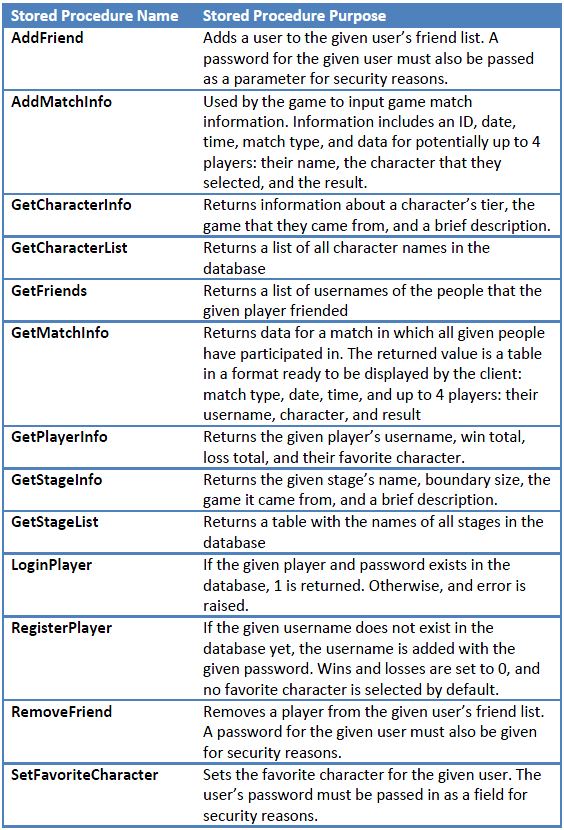
\includegraphics[keepaspectratio, width=5in]{Sprocs.png}\\
\subsection{Indexes}
The only indexes used are the ones that are generated--by default--for the primary keys.
\subsection{Triggers}
There exists a single trigger in the database which ensures that there exist no two players with the same username with distinct capitalization.  All users must have usernames with distinct characters, regardless of capitalization.

\section{Design Analysis}
\subsection{Strengths}
\begin{itemize}
\item The system achieves a high level of security by limiting the user that connects to the database to only run EXEC on the given stored procedures. This prevents people from running unauthorized SQL queries from 3rd party client programs. Also, this makes the system immune to SQL injections.
\item The client hashes the passwords given to it. The password field in the player table is 256 characters long to accept the hashed password.
\item Tables and attributes have intuitive names, with the exception of the Player\_match table. The Player\_match table was a result of normalizing the Match table so that it did not contain any null entries.
\item When changing a player's data, the stored procedures require a password of that player. This is to ensure that one player does not modify another player's data if they were not to use the client and instead use the stored procedures.
\item Stored procedures only examine primary keys of tables when executing, with the exception of passwords. This is to reduce the overhead of secondary indexes.
\item Appropriate referential integrity constraints are in place.
\item Raising errors in the stored procedures helps hide information about the database.
\end{itemize}
\subsection{Weaknesses}
\begin{itemize}
\item The `LoginPlayer' stored procedure is susceptible to brute-force attacks for guessing a password. To mitigate this problem, the stored procedure could only be allowed to run for a given username a certain amount of times per minute.
\item The increased security results in decreased flexibility. The user is limited to only executing stored procedures. If more flexibility is desired, more stored procedures can be added.
\item There is duplicate information on the wins and losses of the player (they are recorded in both the Player table and the Player\_match table). This is to increase performance at the cost of increasing redundancy. If the redundancy is undesired, the wins and losses column in the Player table could be removed, but this would impact performance because a player's wins or losses would have to be counted from the Player\_match table.
\end{itemize}

\section{Appendix A}
\subsection{Relational Schema}
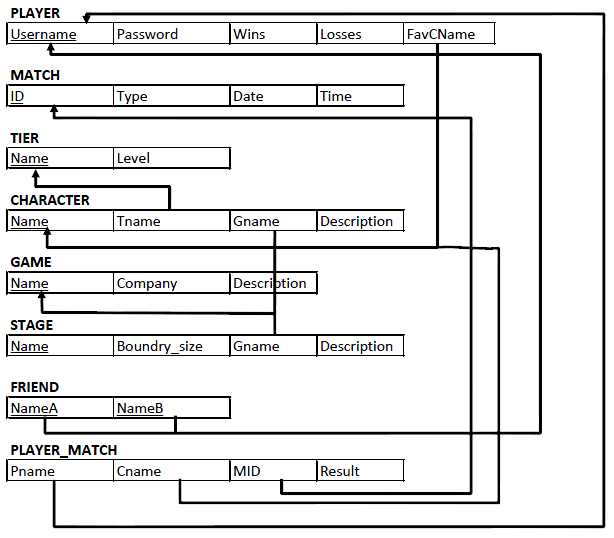
\includegraphics[keepaspectratio, width=6in]{Relational Schema.png}\\
\subsection{Entity Relationship Diagram}
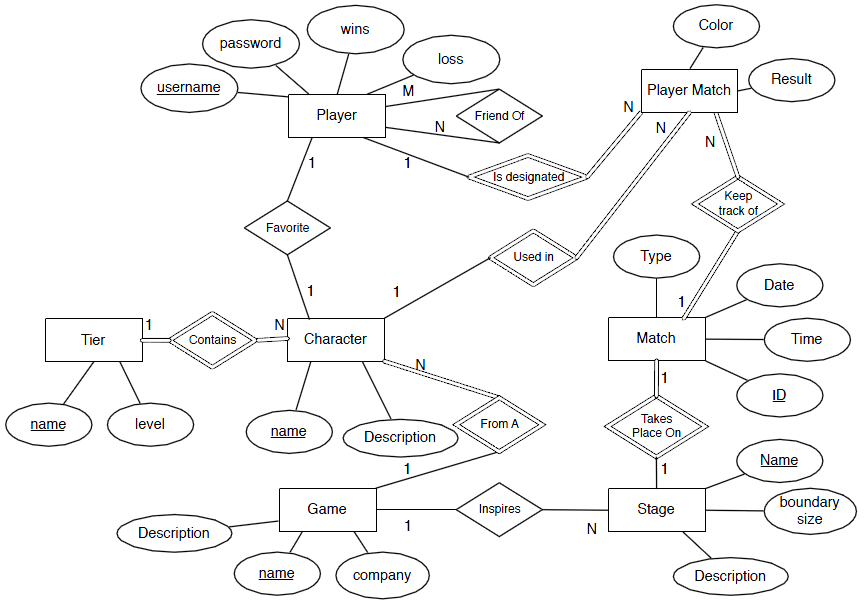
\includegraphics[keepaspectratio, width=6in]{ER.png}\\
\subsection{Explanation of Entity Relationship Diagram}
Each player has a password, an integer for wins, an integer for losses, and a favorite character. Each player can also friend a player, but this relation is directional. Characters can be used to participate in a match, and each character has a name, the game that they came from, and the tier that they belong to. Tiers have a name and a level, which is an integer saying how much better the tier is compared to other tiers (a lower number is better). Matches are kept track of by the database, which have a type, date, time, and participants, which are represented by the Player\_matches table, which keep track of what player participated in what match, what character that they have chosen, and what the result for that player was. Each match takes place on a stage, and each stage has a name, size, and a game that it was inspired from.
\clearpage

\section{Index and Glossary}
\textbf{C\#}: (pronounced 'see pound') multi-paradigm programming language that was developed by Microsoft. (\pageref{csharp}).\\ \\
\textbf{Entity Relationship Diagram}: Abstract and conceptual representation of data. (\pageref{erd}).\\ \\
\textbf{Nintendo Wii}: Seventh generation video game console developed by the Nintendo company. (\pageref{nwii}).\\ \\
\textbf{SSBB}: Super Smash Bros Brawl, a best-selling title for the Nintendo Wii console. (\pageref{ssbb}).\\ \\
\textbf{Visual Studio}: An integrated developer environment developed by Microsoft which is used to create windows applications. (\pageref{vstudio}).\\ \\


\section{References}
\hangindent=1.4cm
\begin{itemize}
\item[1] Super Smash Bros Brawl Smash Nintendo Sales Records. \emph{http://www.nintendo.com/whatsnew/}.
\item[2] Microsoft Visual C\#. \emph{http://msdn.microsoft.com/en-us/vstudio/hh388566}.
\item[3] Microsoft SQL Server 2008. \emph{http://www.microsoft.com/sqlserver/en/us/default.aspx}.
\end{itemize}

\end{document}